% !TeX program = xelatex
% !TeX encoding = UTF-8 Unicode



% ---------------------------------------------------------------- %
% Inonu University FBE Thesis Template - 2025 APA Version           %
%                                                                  %
% Adapted for the 2025 thesis writing guide.                       %
% ---------------------------------------------------------------- %

% ---------------------------------------------------------------- %
% Fill the metadata commands below before writing the thesis text.  %
%                                                                  %
% Based on the Inonu FBE LaTeX thesis template.                    %
%                                                                  %
% Inonu University Graduate School of Natural and Applied Sciences  %
% Malatya, Turkey                                                  %
% https://fenbilimleri.inonu.edu.tr                                         %
% ---------------------------------------------------------------- %
% ------------------------------------------------------------------------------------------------ %
% Main official citation style: APA 7.
% Local adaptation: Inonu FBE 2025 thesis writing guide.           %
% ------------------------------------------------------------------------------------------------ %

% ---------------------------------------------------------------- %
% documentclass options used here:
% [turkce,yukseklisans,bez,fenbilimleri]
% Doktora tezi icin yukseklisans yerine doktora secenegi kullanilmali
% ve ilgili metadata alanlari buna gore doldurulmalidir.
% ---------------------------------------------------------------- %
\documentclass[bez,fenbilimleri,doktora,num,turkce]{inonutez}
\providecommand{\ondalikayirici}[1]{}
\ondalikayirici{nokta}
\providecommand{\sayfaduzeni}[1]{}
\sayfaduzeni{tek}
% ---------------------------------------------------------------- %
% Pay attention to letter case. The structure is case sensitive    %
% {Name}{SURNAME} means first letter of name is capital and that   %
% all letters of surname are capital.                              %
% ---------------------------------------------------------------- %

% ---------------------------------------------------------------- %
% No titles, only Name and SURNAME must be written.      	   %
% ---------------------------------------------------------------- %
\yazar{}{ÖĞRENCİ SOYADI}
\ogrencino{}

% ---------------------------------------------------------------- %
% If you do not use the structure, do not delete it. Just delete   %
% the argument. \unvan{} means title.                              %
% ---------------------------------------------------------------- %
\unvan{}
 
% ---------------------------------------------------------------- %
% For below, the first argument for Turkish, the second is for     %
% English.       						   %
% ---------------------------------------------------------------- %

% ---------------------------------------------------------------- %
% Only the first letters of words must be capital.		   %
% ---------------------------------------------------------------- %
\anabilimdali{Matematik Anabilim Dalı}{Department of Mathematics}
\programi{}{Anabilim dalından otomatik doldurulur Programme}

% ---------------------------------------------------------------- %
% For paperback version, the submission date to the faculty. For   %
% hardcover (indigo/black) version, date of defense.		   %
% ---------------------------------------------------------------- %

\tarih{ARALIK 2024}{DECEMBER 2024}
\tarihKucuk{aralık 2024}{december 2024}

% ---------------------------------------------------------------- %
% Thesis advisor, title, thesis submission date, defense date      %
% ---------------------------------------------------------------- %

% ---------------------------------------------------------------- %
% Add advisor information 
% \tezyoneticisi{}{}
% \tezyoneticisiTR{}{}  --this is required for Turkish cover page fill this in Turkish 
% %
% ---------------------------------------------------------------- %
\tezyoneticisi{}{}
\tezyoneticisiENG{}{}
\bapdestegi{FBA-2026-1234}

% ---------------------------------------------------------------- %
% coadvisor information. If you do not use this,     %
% leave the corresponding arguments blank such as                  %
% \ikincitezdanismani{}{} 					           %
% \esdanismaniTR{}{}   --this is required for Turkish cover page fill this in Turkish  %
% ---------------------------------------------------------------- %
\ikincitezdanismani{Varsa ikinci tez danışmanı}{Varsa ikinci tez danışmanı kurumu}
\ikincitezdanismaniENG{İkinci tez danışmanından otomatik doldurulur}{İkinci tez danışmanı kurumundan otomatik doldurulur}

%Adjust the your thesis title
\baslik{TEZ BAŞLIĞI 1. SATIR}{GEREKLİYSE 2. SATIR}{GEREKLİYSE 3. SATIR}

\title{}{}{}







% ---------------------------------------------------------------- %
% The date of submission of the paperback to the department.	   %
% ---------------------------------------------------------------- %
\tezvermetarih{Eylül 2024}{September 2024}

\tezsavunmatarih{Aralık 2024}{December 2024}
\kapakyili{2025}
\kapaksehri{MALATYA}
\oy{Oy birliği}
\yonetimkurulukarar{22 Eylül 2024}{2024/12}

% ---------------------------------------------------------------- %
% coadvisor and jury information. If you do not use all items,     %
% leave the corresponding arguments blank such as                  %
% \ikincitezdanismani{}{} 					           %
% ---------------------------------------------------------------- %



\juriBir{}{İnönü Üniversitesi}

\juriIki{Jüri 2 Adı Soyadı}{}

\juriUc{Jüri 3 Adı Soyadı}{}

\juriDort{}{İnönü Üniversitesi}

\juriBes{}{İnönü Üniversitesi}

\input defs.tex
\usepackage{docmute}

% ---------------------------------------------------------------- %
% For dedication page. Leave the argument blank if not used.	   %
% ---------------------------------------------------------------- %
\ithaf{}
% ---------------------------------------------------------------- %
% Form the below files						   %
% Scientific WorkPlace/LyX tarafindan tek basina acilabilen bolum dosyalari
% kendi \documentclass ve preamble kisimlarini icerebilir. docmute, ana tez
% derlenirken bu dosyalarin yalnizca document govdesini okur.
% ---------------------------------------------------------------- %
\onsoz{Önsöz bölümü, tezin hazırlanması sürecinde katkı sağlayan
kişi ve kurumlara teşekkür etmek için kullanılır. Bu
bölümde bilimsel içerik tartışılmaz; destek, katkı ve
teşekkür ifadeleri kısa ve açık biçimde yazılır.

Tezi destekleyen kurum adları ve katkı sağlayan kişiler burada
belirtilebilir. Teşekkür edilen kişilerin soyadları büyük
harflerle yazılmalıdır.

Önsöz metninin sonunda, kılavuzdaki yerleşime uygun olarak tarih ve
yazar adı birlikte verilmelidir.
}
\kisaltmalistesi{}
\sembollistesi{\begin{tabular}{@{}p{3cm}l@{}}
\textbf{$\alpha$} & \textbf{:} Alpha \\
\textbf{$\beta$} & \textbf{:} Beta \\
\textbf{AIC} & \textbf{:} Akaike Information Criteria \\
\textbf{ANN} & \textbf{:} Artificial Neural Network \\
\textbf{LaTeX} & \textbf{:} Belge hazirlama sistemi \\
\end{tabular}
}
\ozet{\textbf{Amaç:} Bu dosya, 2025 tez yazım kılavuzuna uygun Türkçe özet yazımı için kısa bir örnektir. Özet metni; tez konusu, amaç, kullanılan yöntem ve ulaşılan temel sonuçları gereksiz ayrıntıya girmeden sunmalıdır.

\textbf{Materyal ve metot:} Bu bölümde araştırma tasarımı, veri kaynağı, deneysel veya kuramsal yöntem ve analiz süreci öz biçimde açıklanır. Özet içinde kaynak, şekil veya tablo verilmez.

\textbf{Bulgular:} Tezin en önemli bulguları doğrudan ve sade bir dille belirtilir. Kısaltmalar gerekiyorsa yalnızca ``Simgeler ve Kısaltmalar Dizini''nde tanımlanan biçimleriyle kullanılmalıdır.

\textbf{Sonuç:} Özet başlık ve anahtar kelimeler hariç en fazla 250 kelime olmalı, tercihen tek sayfaya sığmalıdır. Gerektiğinde satır aralığı 1,15'e indirilebilir.
}
\summary{\textbf{Aim:} This file provides a short sample abstract compatible with the 2025 thesis writing guide. The abstract should state the thesis topic, aim, method, and main conclusions without unnecessary detail.

\textbf{Material and method:} This part briefly describes the research design, data source, experimental or theoretical method, and analysis process. References, figures, and tables should not be included in the abstract.

\textbf{Results:} The most important findings of the thesis are presented directly and clearly. Abbreviations should be used only in the forms defined in the ``Symbols and Abbreviations'' section.

\textbf{Conclusion:} Excluding the title and keywords, the abstract should not exceed 250 words and should preferably fit on a single page. If needed, the line spacing may be reduced to 1.15 only for the abstract pages.
}
\anahtarkelimeler{}
\keywords{}
\etikbeyan{Bu tez çalışmasının hazırlanmasında bilimsel etik
ilkelere ve akademik dürüstlük kurallarına uyduğumu; yararlandığım
tüm kaynakları metin içinde ve kaynaklar bölümünde uygun
biçimde gösterdiğimi beyan ederim.

Bu tez çalışmasında üretken yapay zek\^a tabanlı araçlar
kullanıldıysa, bu araçların hangi amaçla, hangi kapsamda ve
tezin hangi bölümlerinde kullanıldığı danışman bilgisi
dahilinde açıklanmalıdır. Kullanılmadıysa bu cümle,
``Bu tez çalışmasında üretken yapay zek\^a tabanlı araç
kullanılmamıştır.'' şeklinde düzenlenmelidir.
}
\yapayzekakullanimi{hayir}
\yapayzekatablosu{}
\EnstituMuduru{}

\begin{document}

% ---------------------------------------------------------------- %
% Also form the below files. All corresponding inputs should point %
% to a file.                                                       %
% ---------------------------------------------------------------- %
\chapter{G\.{I}R\.{I}\c{S}}

\label{giris} 
%%%%%%%%%%%%%%%%%%%%%%%%%%%%%%%%%%%%%%%%%%%%%%%%%%%%%%%%%%%%%%%%%

Giri\c{s} b\"{o}l\"{u}m\"{u}, tez \c{c}al\i{}\c{s}mas\i{}n\i{}n temel \c{c}er%
\c{c}evesini okuyucuya sunar. Bu b\"{o}l\"{u}mde ara\c{s}t\i{}rma konusu,
problem durumu, tezin amac\i{} ve \"{o}nemi, s\i{}n\i{}rl\i{}l\i{}klar,
varsay\i{}mlar ve temel tan\i{}mlar akademik bir b\"{u}t\"{u}nl\"{u}k i\c{c}%
inde a\c{c}\i{}klanmal\i{}d\i{}r.

K\i{}lavuz gere\u{g}i G\.{I}R\.{I}\c{S} ana ba\c{s}l\i{}\u{g}\i{} alt\i{}nda
ayr\i{}ca numaral\i{} alt ba\c{s}l\i{}k olu\c{s}turulmamal\i{}d\i{}r. Bu
nedenle bu \c{s}ablonda Giri\c{s} b\"{o}l\"{u}m\"{u}, alt ba\c{s}l\i{}k
kullanmadan tek bir ak\i{}\c{s} halinde verilmi\c{s}tir. Gerekli bilgiler,
paragraflar aras\i{}nda mant\i{}kl\i{} ge\c{c}i\c{s}ler kurularak sunulmal\i{%
}; y\"{o}ntem, literat\"{u}r ve bulgulara ili\c{s}kin ayr\i{}nt\i{}lar
ilgili ana b\"{o}l\"{u}mlere b\i{}rak\i{}lmal\i{}d\i{}r.

Bu b\"{o}l\"{u}mde okuyucuya \c{c}al\i{}\c{s}man\i{}n hangi bilimsel bo\c{s}%
lu\u{g}a odakland\i{}\u{g}\i{}, hangi sorulara yan\i{}t arad\i{}\u{g}\i{} ve
tezin genel organizasyonunun nas\i{}l ilerledi\u{g}i k\i{}sa ve a\c{c}\i{}k
bi\c{c}imde aktar\i{}labilir.

\documentclass[12pt,a4paper]{report}
%%%%%%%%%%%%%%%%%%%%%%%%%%%%%%%%%%%%%%%%%%%%%%%%%%%%%%%%%%%%%%%%%
%TCIDATA{OutputFilter=LATEX.DLL}
%TCIDATA{Version=5.50.0.2934}
%TCIDATA{<META NAME="SaveForMode" CONTENT="1">}
%TCIDATA{BibliographyScheme=Manual}
%TCIDATA{<META NAME="DocumentShell" CONTENT="Scientific WorkPlace\LaTeX Report">}
%TCIDATA{Language=Turkish}
%TCIDATA{CSTFile=LaTeX Report.cst}
%TCIDATA{PageSetup=72,72,72,72,0}
%%%%%%%%%%%%%%%%%%%%%%%%%%%%%%%%%%%%%%%%%%%%%%%%%%%%%%%%%%%%%%%%%
\usepackage[utf8]{inputenc}
\usepackage[T1]{fontenc}
\usepackage[shorthands=off,turkish]{babel}
\usepackage{amsmath,amssymb,amsthm}
\usepackage{graphicx}
\usepackage{float}
\usepackage{booktabs}
\usepackage{pdflscape}
\usepackage{caption}
\usepackage{subcaption}
\graphicspath{{./fig/}{fig/}}
\providecommand{\parencite}[1]{(#1)}
\providecommand{\textcite}[1]{#1}
\providecommand{\sekilnotu}[1]{\par\small #1}
\providecommand{\tablonotu}[1]{\par\small #1}
\providecommand{\subsubsubsection}[1]{\paragraph{#1}\mbox{}\\}
\begin{document}
%%%%%%%%%%%%%%%%%%%%%%%%%%%%%%%%%%%%%%%%%%%%%%%%%%%%%%%%%%%%%%%%%
\chapter{GENEL B\.{I}LG\.{I}LER / KURAMSAL \c{C}ER\c{C}EVE}\label{CH2}
%%%%%%%%%%%%%%%%%%%%%%%%%%%%%%%%%%%%%%%%%%%%%%%%%%%%%%%%%%%%%%%%%

\section{Ara\c{s}t\i{}rma Alan\i{}n\i{}n Tan\i{}t\i{}m\i{}}

Bu b\"{o}l\"{u}mde tez konusunun dayand\i{}\u{g}\i{} temel kavramlar, kuramsal yakla\c{s}\i{}mlar ve konu ile ilgili \"{o}nceki \c{c}al\i{}\c{s}malar \"{o}zetlenir. Okuyucunun ara\c{s}t\i{}rma problemini anlayabilmesi i\c{c}in gerekli arka plan bilgisi a\c{c}\i{}k ve sistemli bi\c{c}imde verilir.\footnote{Dipnotlar k\i{}sa tutulmal\i{}; ana metin d\i{}\c{s}\i{}ndaki a\c{c}\i{}klamalar i\c{c}in kullan\i{}lmal\i{}d\i{}r.}

Literat\"{u}r de\u{g}erlendirmesinde yaln\i{}zca kaynaklar\i{} s\i{}ralamak yerine, kaynaklar aras\i{}ndaki ili\c{s}ki, bo\c{s}luk ve tart\i{}\c{s}malara yer verilmelidir. Bu k\i{}s\i{}mda tez \c{c}al\i{}\c{s}mas\i{}n\i{}n hangi bilimsel gereksinimden do\u{g}du\u{g}u ortaya konur \parencite{moore91}.

\section{Kuramsal Yakla\c{s}\i{}mlar}

Kuramsal \c{c}er\c{c}eve, ara\c{s}t\i{}rman\i{}n kulland\i{}\u{g}\i{} kavramlar\i{} ve varsay\i{}mlar\i{} tan\i{}mlar. Metinde kullan\i{}lan her terim, tez boyunca ayn\i{} anlamda kullan\i{}lmal\i{}; zorunlu durumlarda tan\i{}mlar a\c{c}\i{}klanmal\i{}d\i{}r.

\begin{figure}[!ht]
 \centering
 
\includegraphics[width=10cm,keepaspectratio=true]{./fig/sekil2}
 \vspace*{4mm}
 \caption{Kuramsal yap\i{}y\i{} g\"{o}steren \"{o}rnek \c{s}ekil}
 \sekilnotu{Not: \c{S}ekil alt\i{} a\c{c}\i{}klamalar\i{} 9 punto ile verilir.}
 \label{fig:ch2-1}
\end{figure}

\c{S}ekil~\ref{fig:ch2-1}'de g\"{o}sterilen yap\i{}, kuramsal \c{c}er\c{c}evenin temel bile\c{s}enlerini \"{o}zetlemektedir. Metinde \c{s}ekil ve tablolar ilk ge\c{c}tikleri yerde an\i{}lmal\i{}, ard\i{}ndan ilgili g\"{o}rsel verilmelidir.

\section{\.{I}lgili \c{C}al\i{}\c{s}malar}

Bu k\i{}s\i{}mda benzer y\"{o}ntemler, veri kaynaklar\i{} ve bulgular kar\c{s}\i{}la\c{s}t\i{}rmal\i{} olarak ele al\i{}n\i{}r. Kaynak g\"{o}sterimi i\c{c}in uygun at\i{}f komutu kullan\i{}lmal\i{}d\i{}r \parencite{moore91}.

Alt \c{s}ekil kullan\i{}lmas\i{} gerekiyorsa her alt par\c{c}a metinde ayr\i{} ayr\i{} a\c{c}\i{}klanabilir. \c{S}ekil~\ref{fig:ch2-2}'de iki par\c{c}al\i{} bir \c{s}ekil \"{o}rne\u{g}i verilmi\c{s}tir.

\vspace{6pt}
\begin{figure}[ht]
    \centering
    \begin{subfigure}[b]{0.45\textwidth}
        \includegraphics[width=\textwidth]{example-image-a}
        \captionsetup{labelformat=empty}
        \caption*{(a)}
        \label{fig:ch2-2a}
    \end{subfigure}
    \hfill
    \begin{subfigure}[b]{0.45\textwidth}
        \includegraphics[width=\textwidth]{example-image-b}
        \captionsetup{labelformat=empty}
        \caption*{(b)}
        \label{fig:ch2-2b}
    \end{subfigure}
    \caption{Alt \c{s}ekillerden olu\c{s}an ana \c{s}ekil \"{o}rne\u{g}i}
    \label{fig:ch2-2}
\end{figure}

Tablolar, metni gereksiz yere tekrar etmeden veriyi d\"{u}zenli bi\c{c}imde sunmal\i{}d\i{}r. Tablo~\ref{table_ex2}, tez i\c{c}inde kullan\i{}labilecek yal\i{}n bir tablo d\"{u}zenini g\"{o}stermektedir.

\begin{table*}[!ht]
{\setlength{\tabcolsep}{14pt}
\caption{Tablo ba\c{s}l\i{}klar\i{} nokta ile bitmemelidir}
\noindent
\begin{tabular}{cccc}
\hline\hline
Kolon A & Kolon B & Kolon C & Kolon D \\
\hline
Sat\i{}r A & Sat\i{}r A & Sat\i{}r A & Sat\i{}r A \\
Sat\i{}r B & Sat\i{}r B & Sat\i{}r B & Sat\i{}r B \\
Sat\i{}r C & Sat\i{}r C & Sat\i{}r C & Sat\i{}r C \\
\hline
\end{tabular}
\tablonotu{Not: Tablo alt\i{} a\c{c}\i{}klamalar\i{} 9 punto ile verilir.}
\par
\label{table_ex2}}
\end{table*}

Bu b\"{o}l\"{u}m\"{u}n sonunda, kuramsal \c{c}er\c{c}eveden materyal ve metot b\"{o}l\"{u}m\"{u}ne ge\c{c}i\c{s}i sa\u{g}layan k\i{}sa bir de\u{g}erlendirme yap\i{}labilir.
\end{document}

\documentclass[12pt,a4paper]{report}
%%%%%%%%%%%%%%%%%%%%%%%%%%%%%%%%%%%%%%%%%%%%%%%%%%%%%%%%%%%%%%%%%
%TCIDATA{OutputFilter=LATEX.DLL}
%TCIDATA{Version=5.50.0.2934}
%TCIDATA{<META NAME="SaveForMode" CONTENT="1">}
%TCIDATA{BibliographyScheme=Manual}
%TCIDATA{<META NAME="DocumentShell" CONTENT="Scientific WorkPlace\LaTeX Report">}
%TCIDATA{Language=Turkish}
%TCIDATA{CSTFile=LaTeX Report.cst}
%TCIDATA{PageSetup=72,72,72,72,0}
%%%%%%%%%%%%%%%%%%%%%%%%%%%%%%%%%%%%%%%%%%%%%%%%%%%%%%%%%%%%%%%%%
\usepackage[utf8]{inputenc}
\usepackage[T1]{fontenc}
\usepackage[shorthands=off,turkish]{babel}
\usepackage{amsmath,amssymb,amsthm}
\usepackage{graphicx}
\usepackage{float}
\usepackage{booktabs}
\usepackage{pdflscape}
\usepackage{caption}
\usepackage{subcaption}
\graphicspath{{./fig/}{fig/}}
\providecommand{\parencite}[1]{(#1)}
\providecommand{\textcite}[1]{#1}
\providecommand{\sekilnotu}[1]{\par\small #1}
\providecommand{\tablonotu}[1]{\par\small #1}
\providecommand{\subsubsubsection}[1]{\paragraph{#1}\mbox{}\\}
\begin{document}
%%%%%%%%%%%%%%%%%%%%%%%%%%%%%%%%%%%%%%%%%%%%%%%%%%%%%%%%%%%%%%%%%
\chapter{MATERYAL VE METOT}\label{ch:fp}
%%%%%%%%%%%%%%%%%%%%%%%%%%%%%%%%%%%%%%%%%%%%%%%%%%%%%%%%%%%%%%%%%

\section{Ara\c{s}t\i{}rma Materyali}

Bu b\"{o}l\"{u}mde \c{c}al\i{}\c{s}mada kullan\i{}lan veri, deney materyali, yaz\i{}l\i{}m, donan\i{}m, saha bilgisi veya belge kaynaklar\i{} tan\i{}t\i{}l\i{}r. Materyalin nas\i{}l elde edildi\u{g}i, hangi kapsama sahip oldu\u{g}u ve hangi s\i{}n\i{}rl\i{}l\i{}klar\i{} i\c{c}erdi\u{g}i a\c{c}\i{}klanmal\i{}d\i{}r.

\subsection{Veri Kaynaklar\i{}}

Veri kaynaklar\i{} yaz\i{}l\i{}rken tarih aral\i{}\u{g}\i{}, \"{o}rneklem b\"{u}y\"{u}kl\"{u}\u{g}\"{u}, \"{o}l\c{c}\"{u}m birimleri ve veri se\c{c}im \"{o}l\c{c}\"{u}tleri belirtilir. Gerekirse veri haz\i{}rlama s\"{u}reci a\c{s}amalar halinde verilebilir.

\begin{figure}[!ht]
 \centering
 
\includegraphics[width=230pt,keepaspectratio=true]{./fig/sekil3}
 \vspace*{4mm}
 \caption[K\i{}sa \c{s}ekil a\c{c}\i{}klamas\i{}]{Uzun \c{s}ekil a\c{c}\i{}klamas\i{}nda listenin k\i{}sa s\"{u}r\"{u}m\"{u} kullan\i{}labilir}
 \label{fig:3-1-1}
\end{figure}

\c{S}ekil~\ref{fig:3-1-1}, veri veya y\"{o}ntem ak\i{}\c{s}\i{}n\i{} g\"{o}stermek i\c{c}in kullan\i{}labilecek bir g\"{o}rsel \"{o}rne\u{g}idir.

\section{Y\"{o}ntem}

Y\"{o}ntem k\i{}sm\i{}, \c{c}al\i{}\c{s}man\i{}n tekrarlanabilmesini sa\u{g}layacak ayr\i{}nt\i{}da yaz\i{}lmal\i{}d\i{}r. Kullan\i{}lan analiz ad\i{}mlar\i{}, yaz\i{}l\i{}m ayarlar\i{}, varsay\i{}mlar ve de\u{g}erlendirme \"{o}l\c{c}\"{u}tleri burada verilir.

\subsection{Model Kurulumu}

Model veya analiz yakla\c{s}\i{}m\i{} a\c{c}\i{}klan\i{}rken temel denklemler numaraland\i{}r\i{}labilir. Denklem~\ref{eq:3-1}, zaman serisi benzeri bir g\"{o}sterim i\c{c}in \"{o}rnek olarak verilmi\c{s}tir.

\begin{equation}
\label{eq:3-1}
   y_{t}  \equiv \phi_{1} y_{t-1} + \epsilon_{t}
\end{equation}

Denklemden sonra sembollerin anlam\i{} ve modeldeki rolleri metin i\c{c}inde a\c{c}\i{}klanmal\i{}d\i{}r. Daha uzun denklemler gerekiyorsa sat\i{}r k\i{}r\i{}mlar\i{} okunabilirli\u{g}i bozmayacak bi\c{c}imde d\"{u}zenlenmelidir. Birden fazla sat\i{}rda verilen denklemlerde numara son sat\i{}r hizas\i{}nda yer almal\i{}d\i{}r; Denklem~\ref{eq:3-2} bu kullan\i{}ma \"{o}rnektir.

\begin{align}
\widehat{y}_{t}
  &= \beta_{0} + \beta_{1}x_{1t} + \beta_{2}x_{2t} \notag\\
  &\quad + \beta_{3}x_{3t} + \varepsilon_{t}
  \label{eq:3-2}
\end{align}

\subsection{Analiz S\"{u}reci}

Analiz s\"{u}reci; \"{o}n i\c{s}leme, modelleme, do\u{g}rulama ve yorumlama ad\i{}mlar\i{}ndan olu\c{s}abilir. Her ad\i{}m\i{}n amac\i{} ve \c{c}al\i{}\c{s}madaki kar\c{s}\i{}l\i{}\u{g}\i{} a\c{c}\i{}k\c{c}a belirtilmelidir.

\begin{figure}[!ht]
 \centering
 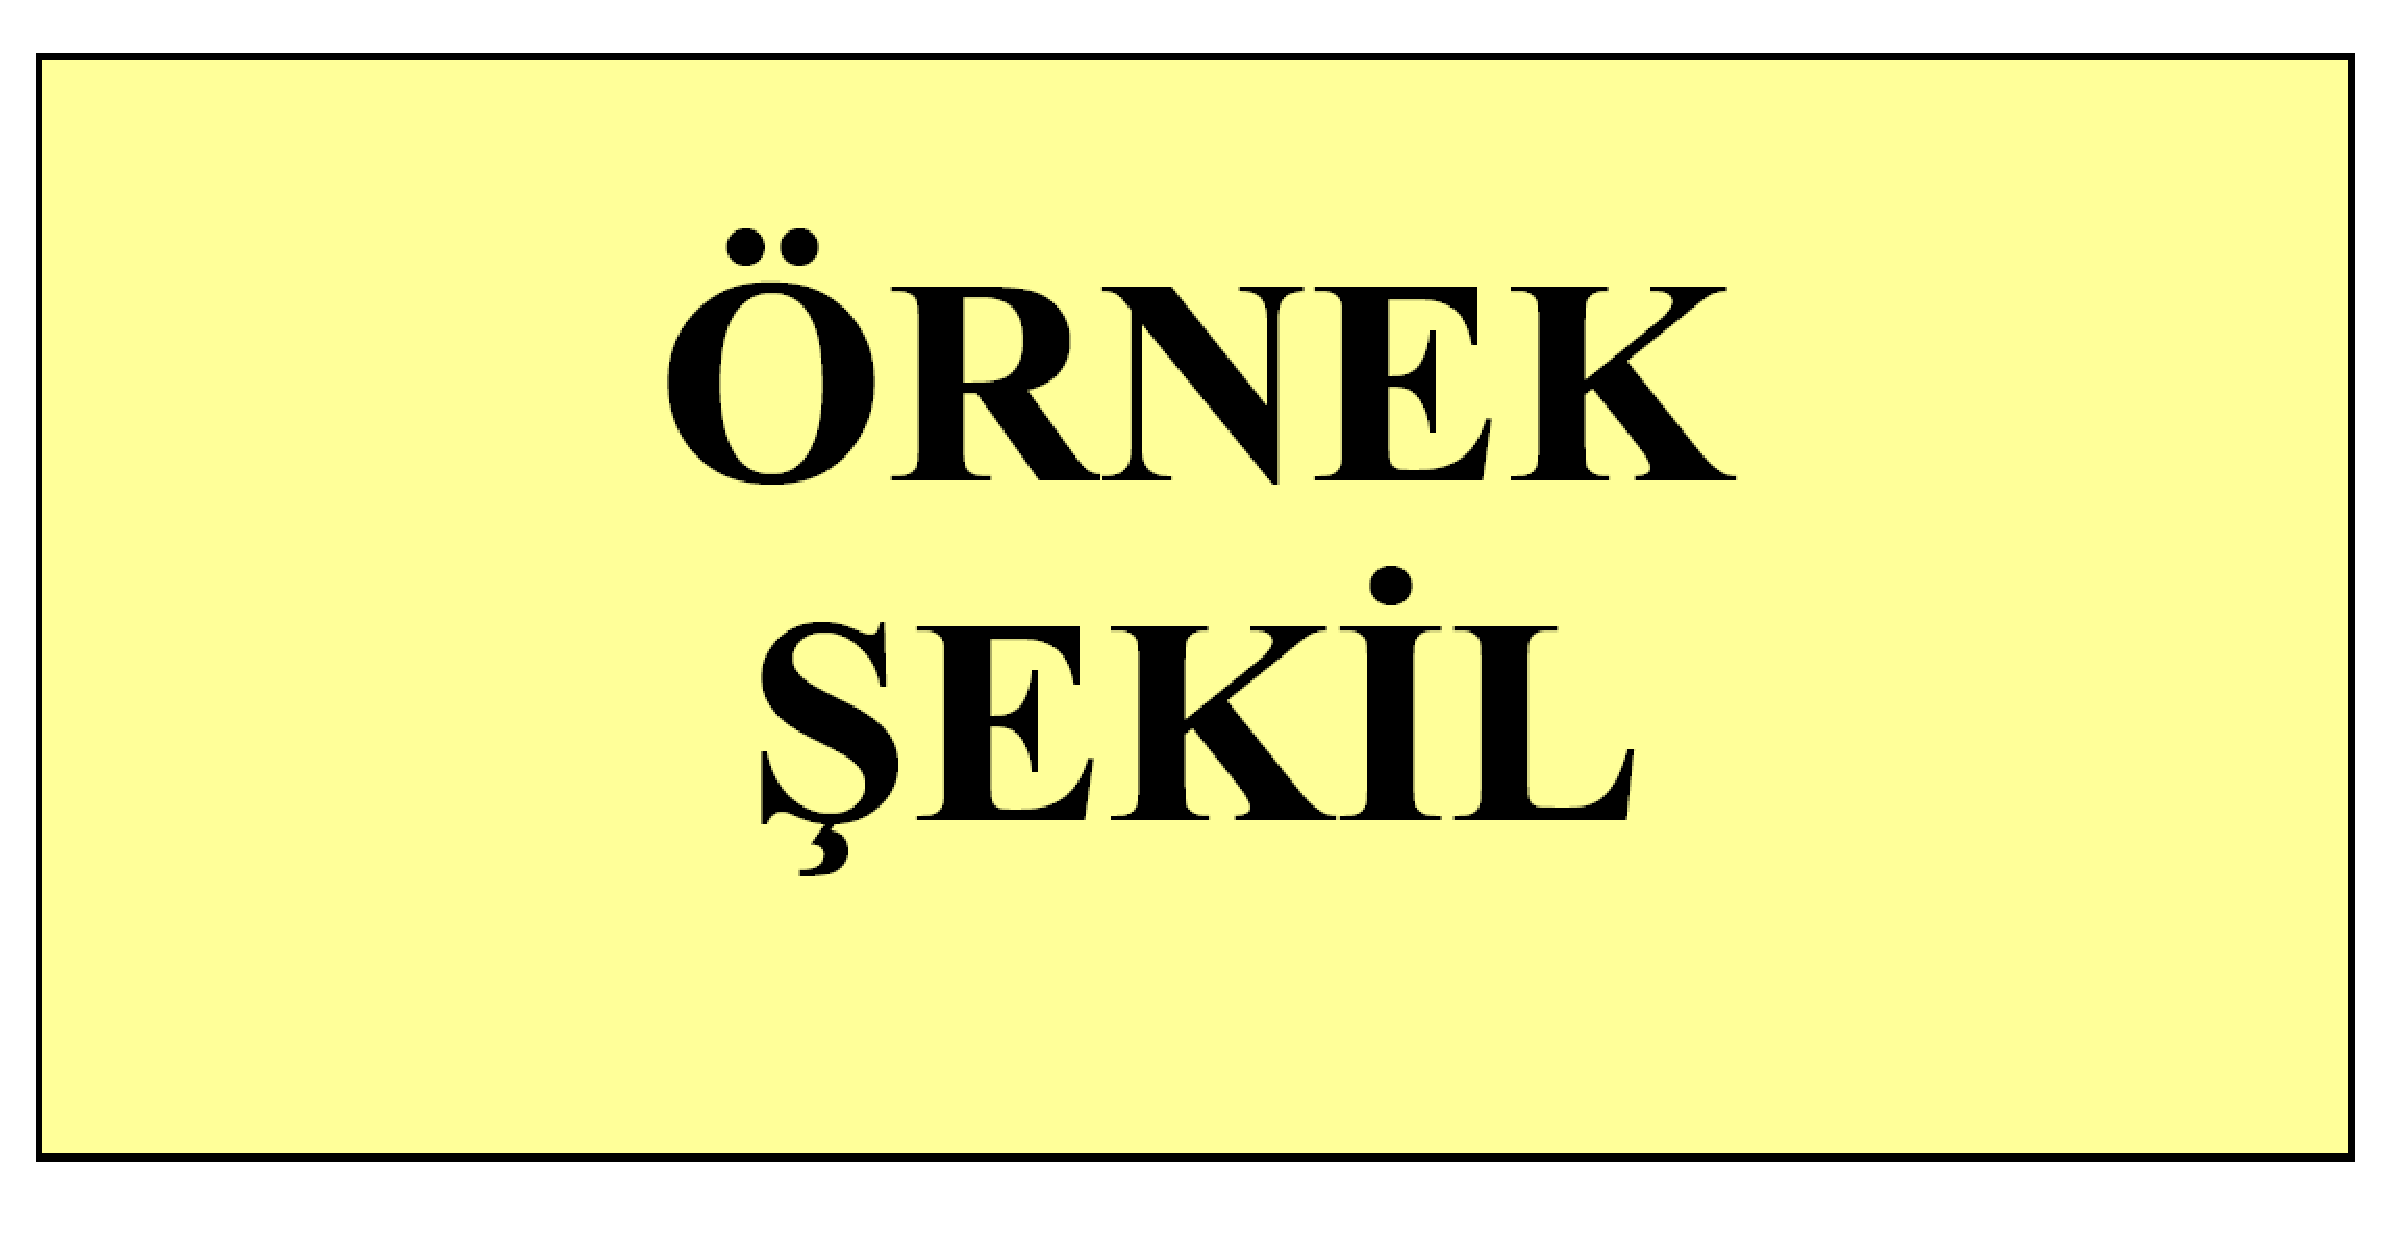
\includegraphics[width=230pt,keepaspectratio=true]{./fig/sekil4}
 \vspace{4mm}
 \caption{\c{C}ok sat\i{}rl\i{} \c{s}ekil a\c{c}\i{}klamalar\i{}nda hizalama \"{o}rne\u{g}i}
 \label{fig:3-1-3}
\end{figure}

\c{S}ekil~\ref{fig:3-1-3}'de y\"{o}ntemin i\c{s} ak\i{}\c{s}\i{} g\"{o}sterilmektedir. \c{S}ekil a\c{c}\i{}klamalar\i{} nokta ile bitirilmemeli ve metin i\c{c}inde ilgili \c{s}ekle mutlaka g\"{o}nderme yap\i{}lmal\i{}d\i{}r.

\section{Yatay Tablo ve \c{S}ekil \"{O}rnekleri}

Sayfaya s\i{}\u{g}mayan tablo veya \c{s}ekiller yatay olarak verilebilir. Yatay kullan\i{}m zorunlu olmad\i{}k\c{c}a tercih edilmemeli, kullan\i{}ld\i{}\u{g}\i{}nda ba\c{s}l\i{}k ve sayfa numaras\i{} yerle\c{s}imi kontrol edilmelidir.

\begin{landscape}
\begin{table}[!ht]
\caption{Yatay sayfada tablo \"{o}rne\u{g}i}
\centering
\begin{tabular}{cccccc}
\hline\hline
De\u{g}i\c{s}ken & A & B & C & D & E \\
\hline
\"{O}rnek 1 & 12 & 18 & 24 & 31 & 35 \\
\"{O}rnek 2 & 14 & 21 & 26 & 33 & 39 \\
\"{O}rnek 3 & 16 & 23 & 29 & 37 & 42 \\
\hline
\end{tabular}
\label{table:landscape_table1}
\end{table}
\end{landscape}

Tablo~\ref{table:landscape_table1}, geni\c{s} i\c{c}erikli tablolar\i{}n yatay sayfada nas\i{}l verilebilece\u{g}ini g\"{o}steren bir \"{o}rnektir.
\end{document}

\documentclass[12pt,a4paper]{report}
%%%%%%%%%%%%%%%%%%%%%%%%%%%%%%%%%%%%%%%%%%%%%%%%%%%%%%%%%%%%%%%%%
%TCIDATA{OutputFilter=LATEX.DLL}
%TCIDATA{Version=5.50.0.2934}
%TCIDATA{<META NAME="SaveForMode" CONTENT="1">}
%TCIDATA{BibliographyScheme=Manual}
%TCIDATA{<META NAME="DocumentShell" CONTENT="Scientific WorkPlace\LaTeX Report">}
%TCIDATA{Language=Turkish}
%TCIDATA{CSTFile=LaTeX Report.cst}
%TCIDATA{PageSetup=72,72,72,72,0}
%%%%%%%%%%%%%%%%%%%%%%%%%%%%%%%%%%%%%%%%%%%%%%%%%%%%%%%%%%%%%%%%%
\usepackage[utf8]{inputenc}
\usepackage[T1]{fontenc}
\usepackage[shorthands=off,turkish]{babel}
\usepackage{amsmath,amssymb,amsthm}
\usepackage{graphicx}
\usepackage{float}
\usepackage{booktabs}
\usepackage{pdflscape}
\usepackage{caption}
\usepackage{subcaption}
\graphicspath{{./fig/}{fig/}}
\providecommand{\parencite}[1]{(#1)}
\providecommand{\textcite}[1]{#1}
\providecommand{\sekilnotu}[1]{\par\small #1}
\providecommand{\tablonotu}[1]{\par\small #1}
\providecommand{\subsubsubsection}[1]{\paragraph{#1}\mbox{}\\}
\begin{document}
%%%%%%%%%%%%%%%%%%%%%%%%%%%%%%%%%%%%%%%%%%%%%%%%%%%%%%%%%%%%%%%%%
\chapter{BULGULAR}\label{ch:ifnecch4}
%%%%%%%%%%%%%%%%%%%%%%%%%%%%%%%%%%%%%%%%%%%%%%%%%%%%%%%%%%%%%%%%%

Bulgular b\"{o}l\"{u}m\"{u}nde, materyal ve metot b\"{o}l\"{u}m\"{u}nde a\c{c}\i{}klanan y\"{o}ntemlerle elde edilen sonu\c{c}lar nesnel bir dille sunulur. Bu b\"{o}l\"{u}mde yorum ve tart\i{}\c{s}ma s\i{}n\i{}rl\i{} tutulmal\i{}; ayr\i{}nt\i{}l\i{} yorumlar tart\i{}\c{s}ma b\"{o}l\"{u}m\"{u}ne b\i{}rak\i{}lmal\i{}d\i{}r.

\section{Bulgular\i{}n Genel De\u{g}erlendirilmesi}

Bu k\i{}s\i{}mda temel bulgular\i{}n genel g\"{o}r\"{u}n\"{u}m\"{u} verilir. Bulgular, ara\c{s}t\i{}rma sorular\i{} veya hipotezlerle ayn\i{} s\i{}ray\i{} izleyecek bi\c{c}imde d\"{u}zenlenebilir.

\subsection{Birinci Veri Seti}

Birinci veri setinden elde edilen bulgular, gerekli tablo ve \c{s}ekillerle desteklenerek sunulur. Metin, tabloda zaten verilen say\i{}lar\i{} tekrar etmek yerine dikkat edilmesi gereken e\u{g}ilimleri a\c{c}\i{}klamal\i{}d\i{}r.

\subsection{\.{I}kinci Veri Seti}

\.{I}kinci veri setine ili\c{s}kin sonu\c{c}lar, ilk veri setiyle kar\c{s}\i{}la\c{s}t\i{}r\i{}labilir. Bulgular aras\i{}ndaki benzerlik ve farklar, tart\i{}\c{s}ma b\"{o}l\"{u}m\"{u}ne temel olu\c{s}turacak bi\c{c}imde belirtilir.

\subsubsection{Model \c{C}\i{}kt\i{}lar\i{}n\i{}n Kar\c{s}\i{}la\c{s}t\i{}r\i{}lmas\i{}}

D\"{o}rd\"{u}nc\"{u} derece ba\c{s}l\i{}klar ancak gerekli oldu\u{g}unda kullan\i{}lmal\i{}d\i{}r. Bu \"{o}rnekte, ayr\i{}nt\i{}l\i{} bir model kar\c{s}\i{}la\c{s}t\i{}rmas\i{}n\i{}n nas\i{}l verilebilece\u{g}i g\"{o}sterilmektedir.

\begin{figure}[!ht]
 \centering
 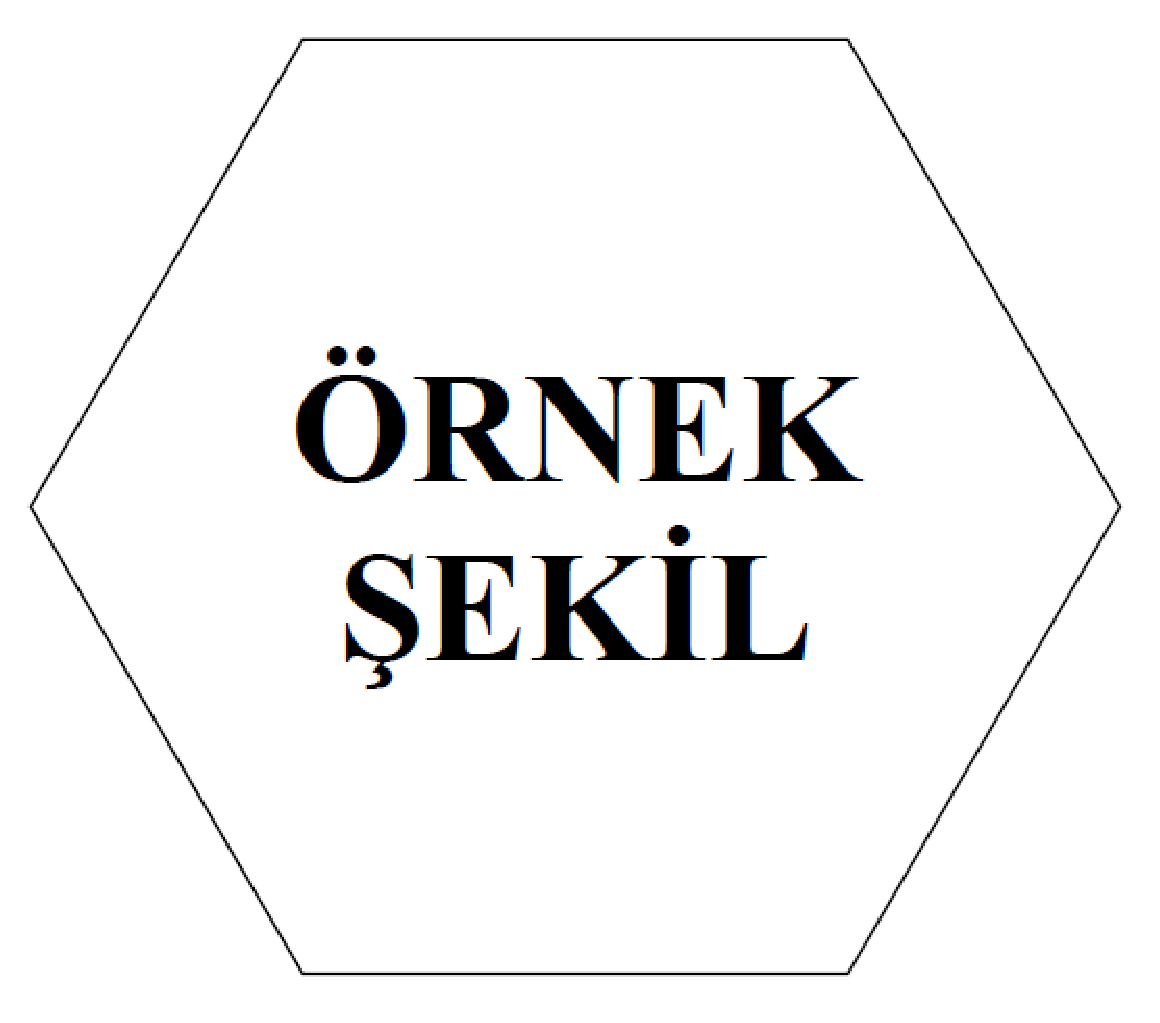
\includegraphics[width=230pt,keepaspectratio=true]{./fig/sekil6}
 \vspace{4mm}
 \caption{\c{C}ok sat\i{}rl\i{} bir \c{s}ekil ba\c{s}l\i{}\u{g}\i{} i\c{c}in hizalama \"{o}rne\u{g}i}
 \label{fig:4-1}
\end{figure}

\c{S}ekil~\ref{fig:4-1}'de bulgular\i{} g\"{o}rselle\c{s}tirmek i\c{c}in kullan\i{}labilecek bir \c{s}ekil d\"{u}zeni verilmi\c{s}tir.

\begin{table*}[!ht]
{\setlength{\tabcolsep}{14pt}
\caption{Bulgular b\"{o}l\"{u}m\"{u}nde \"{o}rnek tablo}
\noindent
\begin{tabular}{cccc}
\hline\hline
Kolon A & Kolon B & Kolon C & Kolon D \\
\hline
Sat\i{}r A & Sat\i{}r A & Sat\i{}r A & Sat\i{}r A \\
Sat\i{}r B & Sat\i{}r B & Sat\i{}r B & Sat\i{}r B \\
Sat\i{}r C & Sat\i{}r C & Sat\i{}r C & Sat\i{}r C \\
\hline
\end{tabular}
\par
\label{tableforCh4-1}}
\end{table*}

Tablo~\ref{tableforCh4-1}, bulgular\i{}n tablo i\c{c}inde nas\i{}l d\"{u}zenlenebilece\u{g}ini g\"{o}steren k\i{}sa bir \"{o}rnektir.
\end{document}

\documentclass[12pt,a4paper]{report}
%%%%%%%%%%%%%%%%%%%%%%%%%%%%%%%%%%%%%%%%%%%%%%%%%%%%%%%%%%%%%%%%%
%TCIDATA{OutputFilter=LATEX.DLL}
%TCIDATA{Version=5.50.0.2934}
%TCIDATA{<META NAME="SaveForMode" CONTENT="1">}
%TCIDATA{BibliographyScheme=Manual}
%TCIDATA{<META NAME="DocumentShell" CONTENT="Scientific WorkPlace\LaTeX Report">}
%TCIDATA{Language=Turkish}
%TCIDATA{CSTFile=LaTeX Report.cst}
%TCIDATA{PageSetup=72,72,72,72,0}
%%%%%%%%%%%%%%%%%%%%%%%%%%%%%%%%%%%%%%%%%%%%%%%%%%%%%%%%%%%%%%%%%
\usepackage[utf8]{inputenc}
\usepackage[T1]{fontenc}
\usepackage[shorthands=off,turkish]{babel}
\usepackage{amsmath,amssymb,amsthm}
\usepackage{graphicx}
\usepackage{float}
\usepackage{booktabs}
\usepackage{pdflscape}
\usepackage{caption}
\usepackage{subcaption}
\graphicspath{{./fig/}{fig/}}
\providecommand{\parencite}[1]{(#1)}
\providecommand{\textcite}[1]{#1}
\providecommand{\sekilnotu}[1]{\par\small #1}
\providecommand{\tablonotu}[1]{\par\small #1}
\providecommand{\subsubsubsection}[1]{\paragraph{#1}\mbox{}\\}
\begin{document}
%%%%%%%%%%%%%%%%%%%%%%%%%%%%%%%%%%%%%%%%%%%%%%%%%%%%%%%%%%%%%%%%%
\chapter{TARTI\c{S}MA}\label{ch:ifnecch5}
%%%%%%%%%%%%%%%%%%%%%%%%%%%%%%%%%%%%%%%%%%%%%%%%%%%%%%%%%%%%%%%%%

Tart\i{}\c{s}ma b\"{o}l\"{u}m\"{u}, bulgular\i{}n yaln\i{}zca tekrar edildi\u{g}i bir b\"{o}l\"{u}m olmamal\i{}d\i{}r. Bu b\"{o}l\"{u}mde bulgular\i{}n anlam\i{}, literat\"{u}rle ili\c{s}kisi, beklenen veya beklenmeyen y\"{o}nleri ve \c{c}al\i{}\c{s}man\i{}n s\i{}n\i{}rl\i{}l\i{}klar\i{} ele al\i{}n\i{}r.

\section{\c{C}al\i{}\c{s}man\i{}n Uygulama Alan\i{}}

Elde edilen sonu\c{c}lar\i{}n hangi alanlarda kullan\i{}labilece\u{g}i, hangi ko\c{s}ullarda ge\c{c}erli oldu\u{g}u ve hangi durumlarda dikkatli yorumlanmas\i{} gerekti\u{g}i a\c{c}\i{}klan\i{}r.

\section{Bulgular\i{}n Literat\"{u}rle Kar\c{s}\i{}la\c{s}t\i{}r\i{}lmas\i{}}

Bu k\i{}s\i{}mda bulgular, ilgili \c{c}al\i{}\c{s}malarla benzerlik ve farkl\i{}l\i{}klar\i{} a\c{c}\i{}s\i{}ndan tart\i{}\c{s}\i{}l\i{}r. Kaynaklara yap\i{}lan g\"{o}ndermeler tart\i{}\c{s}man\i{}n ak\i{}\c{s}\i{}na hizmet etmelidir \parencite{Zuckerman199486}.

\subsection{Y\"{o}ntemin S\i{}n\i{}rl\i{}l\i{}klar\i{}}

Her y\"{o}ntemin varsay\i{}mlar\i{} ve s\i{}n\i{}rl\i{}l\i{}klar\i{} vard\i{}r. Veri kapsam\i{}, \"{o}rneklem, \"{o}l\c{c}\"{u}m do\u{g}rulu\u{g}u, model se\c{c}imi veya yorumlama s\i{}n\i{}rlar\i{} burada a\c{c}\i{}k\c{c}a belirtilmelidir.

\subsubsection{Gelecek \c{C}al\i{}\c{s}malara Etkisi}

Bulgular\i{}n hangi yeni ara\c{s}t\i{}rma sorular\i{}n\i{} do\u{g}urdu\u{g}u ve sonraki \c{c}al\i{}\c{s}malar i\c{c}in nas\i{}l bir yol haritas\i{} sundu\u{g}u a\c{c}\i{}klanabilir.

\subsubsubsection{Ek De\u{g}erlendirme Ba\c{s}l\i{}\u{g}\i{}}

D\"{o}rd\"{u}nc\"{u} dereceden sonraki ba\c{s}l\i{}klar zorunlu olmad\i{}k\c{c}a kullan\i{}lmamal\i{}; kullan\i{}ld\i{}\u{g}\i{}nda numaras\i{}z ve dizinde yer almayan yard\i{}mc\i{} ba\c{s}l\i{}k olarak kalmal\i{}d\i{}r.

\begin{figure}[!ht]
 \centering
 
\includegraphics[width=230pt,keepaspectratio=true]{./fig/sekil5}
 \vspace{4mm}
 \caption{Tart\i{}\c{s}ma b\"{o}l\"{u}m\"{u}nde kullan\i{}labilecek \"{o}rnek \c{s}ekil}
 \label{fig:5-1}
\end{figure}

\c{S}ekil~\ref{fig:5-1}'de tart\i{}\c{s}ma kapsam\i{}nda kullan\i{}labilecek bir g\"{o}rsel \"{o}rne\u{g}i verilmi\c{s}tir.

\begin{table*}[!ht]
{\setlength{\tabcolsep}{14pt}
\caption{Tart\i{}\c{s}ma b\"{o}l\"{u}m\"{u}nde \"{o}rnek tablo}
\noindent
\begin{tabular}{cccc}
\hline\hline
Kolon A & Kolon B & Kolon C & Kolon D \\
\hline
Sat\i{}r A & Sat\i{}r A & Sat\i{}r A & Sat\i{}r A \\
Sat\i{}r B & Sat\i{}r B & Sat\i{}r B & Sat\i{}r B \\
Sat\i{}r C & Sat\i{}r C & Sat\i{}r C & Sat\i{}r C \\
\hline
\end{tabular}
\par
\label{tableforCh5-1}}
\end{table*}

Tablo~\ref{tableforCh5-1}, tart\i{}\c{s}ma b\"{o}l\"{u}m\"{u}nde say\i{}sal \"{o}zetlerin nas\i{}l verilebilece\u{g}ini g\"{o}stermektedir.
\end{document}

\documentclass[12pt,a4paper]{report}
%%%%%%%%%%%%%%%%%%%%%%%%%%%%%%%%%%%%%%%%%%%%%%%%%%%%%%%%%%%%%%%%%
%TCIDATA{OutputFilter=LATEX.DLL}
%TCIDATA{Version=5.50.0.2934}
%TCIDATA{<META NAME="SaveForMode" CONTENT="1">}
%TCIDATA{BibliographyScheme=Manual}
%TCIDATA{<META NAME="DocumentShell" CONTENT="Scientific WorkPlace\LaTeX Report">}
%TCIDATA{Language=Turkish}
%TCIDATA{CSTFile=LaTeX Report.cst}
%TCIDATA{PageSetup=72,72,72,72,0}
%%%%%%%%%%%%%%%%%%%%%%%%%%%%%%%%%%%%%%%%%%%%%%%%%%%%%%%%%%%%%%%%%
\usepackage[utf8]{inputenc}
\usepackage[T1]{fontenc}
\usepackage[shorthands=off,turkish]{babel}
\usepackage{amsmath,amssymb,amsthm}
\usepackage{graphicx}
\usepackage{float}
\usepackage{booktabs}
\usepackage{pdflscape}
\usepackage{caption}
\usepackage{subcaption}
\graphicspath{{./fig/}{fig/}}
\providecommand{\parencite}[1]{(#1)}
\providecommand{\textcite}[1]{#1}
\providecommand{\sekilnotu}[1]{\par\small #1}
\providecommand{\tablonotu}[1]{\par\small #1}
\providecommand{\subsubsubsection}[1]{\paragraph{#1}\mbox{}\\}
\begin{document}
%%%%%%%%%%%%%%%%%%%%%%%%%%%%%%%%%%%%%%%%%%%%%%%%%%%%%%%%%%%%%%%%%
\chapter{SONU\c{C} VE \"{O}NER\.{I}LER}\label{ch:ch6}
%%%%%%%%%%%%%%%%%%%%%%%%%%%%%%%%%%%%%%%%%%%%%%%%%%%%%%%%%%%%%%%%%

Bu b\"{o}l\"{u}mde \c{c}al\i{}\c{s}man\i{}n temel sonu\c{c}lar\i{} k\i{}sa, a\c{c}\i{}k ve b\"{u}t\"{u}nl\"{u}kl\"{u} bi\c{c}imde sunulur. Bulgular b\"{o}l\"{u}m\"{u}ndeki ayr\i{}nt\i{}lar tekrar edilmemeli; ara\c{s}t\i{}rma sorular\i{}na verilen yan\i{}tlar \"{o}ne \c{c}\i{}kar\i{}lmal\i{}d\i{}r.

\section{Sonu\c{c}lar\i{}n De\u{g}erlendirilmesi}

Tez kapsam\i{}nda elde edilen sonu\c{c}lar, ara\c{s}t\i{}rman\i{}n amac\i{} ile ili\c{s}kilendirilerek a\c{c}\i{}klan\i{}r. Bu k\i{}s\i{}m, okuyucuya \c{c}al\i{}\c{s}man\i{}n bilimsel katk\i{}s\i{}n\i{} toplu olarak g\"{o}stermelidir.

\subsection{Ara\c{s}t\i{}rma Bulgular\i{}na Dayal\i{} Sonu\c{c}lar}

Temel bulgular\i{}n her biri, k\i{}sa ve do\u{g}rudan c\"{u}mlelerle belirtilir. Bulgular\i{}n hangi veri, analiz veya g\"{o}zleme dayand\i{}\u{g}\i{} gerekti\u{g}inde hat\i{}rlat\i{}labilir.

\subsubsection{Y\"{o}nteme \.{I}li\c{s}kin Sonu\c{c}lar}

Y\"{o}ntemin \c{c}al\i{}\c{s}maya sa\u{g}lad\i{}\u{g}\i{} katk\i{}, g\"{u}\c{c}l\"{u} y\"{o}nleri ve s\i{}n\i{}rlar\i{} burada \"{o}zetlenebilir.

\subsubsubsection{Ek Sonu\c{c} Notu}

Bu ba\c{s}l\i{}k, d\"{o}rd\"{u}nc\"{u} dereceden sonra kullan\i{}lan numaras\i{}z yard\i{}mc\i{} ba\c{s}l\i{}k \"{o}rne\u{g}idir.

\begin{figure}[!ht]
 \centering
 
\includegraphics[width=230pt,keepaspectratio=true]{./fig/sekil7}
 \vspace{4mm}
 \caption{Sonu\c{c} b\"{o}l\"{u}m\"{u}nde \"{o}rnek \c{s}ekil}
 \label{fig:6-1}
\end{figure}

\c{S}ekil~\ref{fig:6-1}, sonu\c{c} b\"{o}l\"{u}m\"{u}nde kullan\i{}labilecek \"{o}zet bir g\"{o}rsel i\c{c}in yer tutucu olarak verilmi\c{s}tir.

\begin{table*}[!ht]
{\setlength{\tabcolsep}{14pt}
\caption{Sonu\c{c} b\"{o}l\"{u}m\"{u}nde \"{o}rnek tablo}
\noindent
\begin{tabular}{cccc}
\hline\hline
Kolon A & Kolon B & Kolon C & Kolon D \\
\hline
Sat\i{}r A & Sat\i{}r A & Sat\i{}r A & Sat\i{}r A \\
Sat\i{}r B & Sat\i{}r B & Sat\i{}r B & Sat\i{}r B \\
Sat\i{}r C & Sat\i{}r C & Sat\i{}r C & Sat\i{}r C \\
\hline
\end{tabular}
\par
\label{tableforCh6-1}}
\end{table*}

Tablo~\ref{tableforCh6-1}, sonu\c{c}lar\i{}n \"{o}zetlenmesi i\c{c}in kullan\i{}labilecek basit bir tablo d\"{u}zenidir.

\section{\"{O}neriler}

\"{O}neriler, \c{c}al\i{}\c{s}man\i{}n sonu\c{c}lar\i{}na dayanmal\i{} ve uygulanabilir nitelikte olmal\i{}d\i{}r. Yeni ara\c{s}t\i{}rmalar, y\"{o}ntem geli\c{s}tirmeleri veya uygulama alanlar\i{} i\c{c}in somut \"{o}neriler bu k\i{}s\i{}mda verilebilir.
\end{document}


% APA references are read from kaynaklar.bib. Use \parencite or \textcite.



\makeatletter
\if@APAStyle
  \setlength\bibitemsep{0pt}
  \printbibliography[heading=bibliography]
\else
  \bibliographystyle{inonubib}
  \bibliography{kaynaklar}
\fi
\makeatother

% ---------------------------------------------------------------- %
% Appendix files. eklerkapak is the appendix title page.           %
% ---------------------------------------------------------------- %
\eklerkapak{}
\input eklerkapak.tex  

% ---------------------------------------------------------------- %
% \eklerbolum{x} forms and appendix of x chapters. 
% ---------------------------------------------------------------- %
\eklerbolum{0}
\chapter{EK-1 Özgeçmiş}
\input ozgecmis.tex
\input ekler.tex

% ---------------------------------------------------------------- %
% Ozgecmis is printed as EK-1 in the appendices for the 2025 guide. %
% ---------------------------------------------------------------- %
\ozgecmissondabasmasin
\end{document}                      

% ---------------------------------------------------------------- %
% About this template: Inonu University FBE adaptation              %
% ---------------------------------------------------------------- %
